\setchapterpreamble[u]{\margintoc}
\chapter{Fruit Ninja GL}

\begin{chap-intro}
	In questo capitolo si descriverà nel dettaglio il progetto d'esame, effettuando prima una breve overview sulle principali caratteristiche e scelte implementative ed architetturali per poi successivamente passare ai vari dettagli implementativi.
\end{chap-intro}

\section{Overview}
Fruit Ninja GL è basato in OpenGL 4.6 Core Profile utilizzando la libreria GLFW 3.3.2 per la crazione del contesto, finestra e gestione di input ed eventi. L'applicazione è stata sviluppata in C++20 in ambiente Visual Studio\sidenote{Il codice è compilabile in ambiente linux utilizzando un altro compilatore.} 2019.

\subsubsection{Simile all'originale}
\begin{marginfigure}
	\centering
	
\includegraphics[width=0.7\linewidth]{images/ch20/0}
	\caption{Esempio di sprite realizzato imitando lo stile di Fruit Ninja.}
	\label{fig:combo4}
\end{marginfigure}
Durante lo sviluppo si è cercati di rimanere il più possibile fedeli al gioco nella sua versione originale rilasciata nel 2010. Musiche, suoni, font e sfondi sono liberamente disponibili in rete mentre gli sprite ed elementi della GUI sono stati riprodotti utilizzando photoshop\footnote{Tutti i file \texttt{.psd} creati ed utilizzati sono inclusi assieme agli asset.}.

I modelli 3D dei frutti sia nella loro versione \enquote{intera} che \enquote{affettata} sono presi da uno dei tanti Fruit pack disponibili in rete.


\subsubsection{Entity Component System}
Lo sviluppo delle logiche di gioco è stato basato sull'Entity Component System, un pattern architetturale molto comune nel game development\sidenote{Utilizzabile in molti motori grafici come Unity, Unreal Engine o il Cryengine.}


\subsubsection{Astrazione delle primitive}
Tutte le principali primitive grafiche (di OpenGL e non) come \textit{texture}, \textit{mesh}, \textit{model}, \textit{shader} o \textit{audio} sono state astratte in specifiche classi per rendere più semplice, immediato e conveniente il loro utilizzo.


\subsubsection{VAOs, VBOs, Vertex e Shaders}
\marginnote{
Si è scelto questo approccio invece che la semplice \textit{direct API mode} (\texttt{glBegin()}, \texttt{glEnd()}, ...) perché quest'ultima è deprecata (e dunque nemmeno disponibile nel  Core Profile), molto più lenta oltre che poco \enquote{compatibile} con il loading di asset e modelli 3D complessi.
}
Il rendering dei vari oggetti è effettuato ricorrendo ai vari buffer (Vertex Array Object, Vertex Buffer Array, Index Buffer Array) e Shaders (Vertex e Fragment) di OpenGL. Sono stati implementati diversi shader a seconda dell'elemento grafico o di come lo si vuole disegnare nel framebuffer.

Dopo una iniziale difficoltà l'utilizzo dei buffer unito con gli shader rende lo sviluppo più semplice e flessibile.


\subsubsection{Engine a Stati}
L'engine di gioco è basato sul Game State 'Stack' un altro pattern architetturale molto diffuso per la gestione dei vari possibili stati di gioco (Loading, playng, pause, game over, ...).


\section{Descrizione Architetturale}
Architetturalmente Fruit Ninja GL è strutturato in cinque \textit{macro-moduli} ognuno dei quali si occupa di gestire una parte dell'applicazione. 
\begin{itemize}
	\item \texttt{core/} classi finalizzate alla gestione dei dettagli a basso livello di OpenGL e non.
	\item \texttt{ecs/} implementazione dell'ECS con componenti, sistemi e relative classi di gestione delle entità.
	\item \texttt{engine/} implementazione del motore di gioco a stati.
	\item \texttt{logic/} dettagli relativi al gameplay e agli elementi di gioco.
	\item \texttt{utl/} classi e funzioni di utility o debug.
\end{itemize}

\subsection{Modulo \texttt{core/}}
Il modulo \texttt{core} contiene tutta una serie di classi e funzioni con il principale scopo di astrarre il più possibile le funzionalità a basso livello messe a disposizione da OpenGL e da altre librerie. L'idea è quella di creare una serie di API semplici su cui si baserà l'intera applicazione.

\begin{figure}[!hpt]
	\centering
	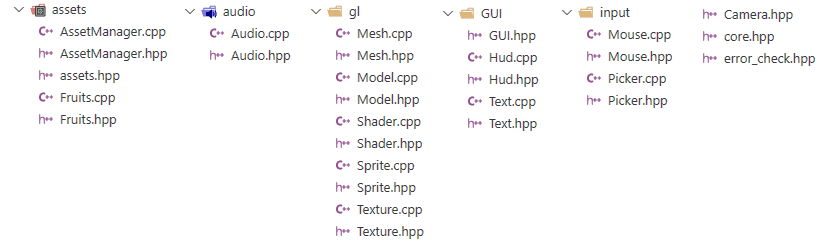
\includegraphics[width=\linewidth]{images/ch20/1}
	\caption{Sotto-moduli e relativi file \texttt{.hpp} e \texttt{.cpp} che fanno parte di \texttt{core}.}
	\label{fig:module-core}
\end{figure}

Come è possibile vedere in figura \rref{fig:module-core} \texttt{core} è strutturato in sotto-moduli ognuno con funzionalità specifiche; nella root principale invece è presente:
\begin{itemize}
\item \texttt{Camera.hpp} una semplice classe che gestisce la camera posizionandola nello spazio e costruendo di conseguenza la \textit{projection matrix} (prospettica) e la \textit{view matrix}.
\item \texttt{error\_check.hpp} contiene macro e callback per il debug ed il checking di errori di OpenGL.
\end{itemize}

\subsubsection{Sotto-modulo \texttt{asset}}
\begin{marginfigure}%[!hpt]
	\centering
	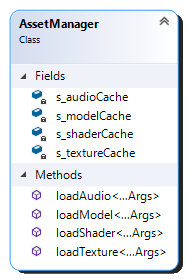
\includegraphics[width=0.8\linewidth]{images/ch20/2}
	\caption{Diagramma UML della classe AssetManager}
\end{marginfigure}
Dedicato alla gestione di asset e risorse grafiche/multimediali di gioco. Oltre alla semplice definizione di cartelle e percorsi (\texttt{asset.hpp}) o alla strutturazione di asset composti (\texttt{fruit.hpp}) nel modulo si implementa anche un \textit{gestore degli asset} (\texttt{AssetManager.hpp}) che utilizzando il patter flyweight consente di caricare e riutilizzare in maniera veloce e dinamica le varie risorse di gioco fornendo lo stesso puntatore ogni qual volta quella risorsa è richiesta.

Tutti gli asset inoltre hanno costruttori di copia e assegnazione disabilitati per evitare duplicazione di risorse.

\begin{cpp}[caption={Esempio di metodo utilizzata dal manager per il caricamento dei Modelli.}, captionpos=t]
template<typename ...Args>
inline constexpr ModelSP AssetManager::loadModel(const fs::path& filepath, Args && ...args)
{
	// Verifico che il modello non sia in cache
	auto f = filepath.string();
	if (AssetManager::s_modelCache.find(f) != AssetManager::s_modelCache.end())
	return AssetManager::s_modelCache[f];
	
	auto model = std::make_shared<Model>(filepath, std::forward<Args>(args)...);
	AssetManager::s_modelCache[f] = model;
	return model;
}
\end{cpp}


\subsubsection{Sotto-modulo \texttt{audio}}
Dedicato alla gestione delle funzionalità audio sia 2D che 3D dell'{}applicazione ricorrendo alla libreria irrKlang \cite{IRRKLANG}. La classe \texttt{Audio} è considerata come un asset di gioco, si occupa del caricamento nonché dell'esecuzione dei file audio e fornisce metodi statici per la gestione generale\sidenote{Ad esempio per interrompere tutti i suoni in esecuzione o semplicemente abbassare il volume.}.


\subsubsection{Sotto-modulo \texttt{gl}}
Dedicato all'astrazione delle principali primitive di OpenGL in modo da consentine un uso facile e componibile. 
\begin{itemize}
\item \texttt{Texture}: gestisce il loading, creazione e binding delle texture. Il caricamento del file in sè avviene tramite la libreria \texttt{stb\_image} \cite{STB} mentre la creazione e binding openGL è effettuato al caricamento supporta anche eventuali parametri. La classe è anche un asset.
\begin{cpp}
Texture::Parameteri parm = {
	{ GL_TEXTURE_WRAP_S, GL_MIRRORED_REPEAT },
	{ GL_TEXTURE_WRAP_T, GL_MIRRORED_REPEAT },
	{ GL_TEXTURE_MIN_FILTER, GL_NEAREST },
	{ GL_TEXTURE_MAG_FILTER, GL_NEAREST },
};
this->m_texture = AssetManager::loadTexture(filepath, parm);
\end{cpp}

\item \texttt{Mesh}: gestisce una singola Mesh + texture. I dati sono rappresentati utilizzando le strutture e buffer di OpenGL. La classe definisce anche la struttura e layout dei vertici\sidenote{Tale struttura è quella che poi è utilizzata in ogni elemento 3D.}.

\item \texttt{Model}: gestisce un Modello, ovvero una composizione di più mesh. Il caricamento dei modelli dal disco avviene utilizzando la libreria ASSIMP \cite{ASSIMP}.

\item \texttt{Shader}: gestisce gli shader\sidenote{Uno \texttt{Shader} è composto da un vertex shader e da un fragment shader.} di OpenGL, la classe ne consente il caricamento del sorgente \texttt{.glsl}, la compilazione, il linking ed in fine l'attivazione o disattivazione.
\end{itemize}

\subsubsection{Sotto-modulo \texttt{input}}
Dedicato alla gestione degli input utente. 
\begin{itemize}
	\item \texttt{Mouse}, singleton tramite il quale ogni altro componente può sapere quale pulsante è stato premuto e le ultime posizioni assunte dal mouse durante il trascinamento nella finestra creata da GLFW.
	\item \texttt{Picker}, classe speciale che consente di effettuare il picking delle entità disegnate sul framebuffer.
\end{itemize}


\subsection{Modulo \texttt{ecs/}}
Il modulo \texttt{ecs} implementa il pattern architetturale Entity Component System.

\begin{figure}[!hpt]
	\centering
	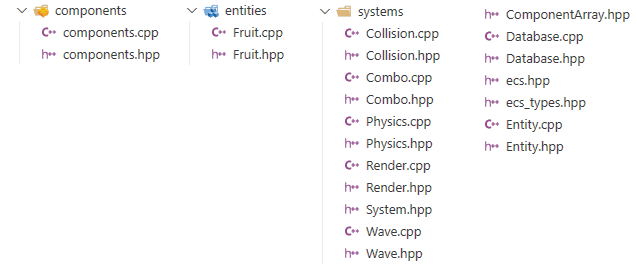
\includegraphics[width=0.95\linewidth]{images/ch20/3}
	\caption{Sotto-moduli e relativi file \texttt{.hpp} e \texttt{.cpp} che fanno parte di \texttt{ecs}.}
	\label{fig:module-ecs}
\end{figure}

Il funzionamento, le classi e eventuali dettagli implementativi verranno descritti nella sezione \rref{sec::ecs}.


\subsection{Modulo \texttt{engine/}}
Il modulo \texttt{engine} implementa il pattern architetturale Game state ``stack" per la gestione degli stati di gioco ed il game loop.

\begin{figure}[!hpt]
	\centering
	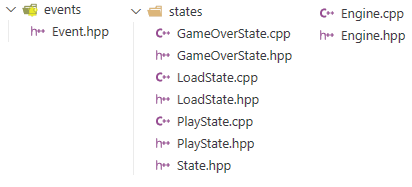
\includegraphics[width=0.8\linewidth]{images/ch20/4}
	\caption{Sotto-moduli e relativi file \texttt{.hpp} e \texttt{.cpp} che fanno parte di \texttt{engine}.}
	\label{fig:module-engine}
\end{figure}

La classe principale per il funzionamento di tutta l'applicazione è \texttt{Engine} ovvero il motore di gioco. Engine è un singleton che ha il compito di inizializzare l'intera applicazione (moduli, sotto-moduli, contesti e librerie) per poi avviare il game loop sullo stato correntemente in cima allo stack degli stati.

\begin{cpp}[caption={Funzione che esegue un singolo loop di gioco. Una volta determinato il 
 tempo trascorso dall'ultima iterazione in ordine: si effettua il polling degli eventi (glfw), si gestisce l'input, si aggiorna lo stato interno, si effettua il rendering ed in fine si gestiscono gli eventi di gioco.
}, captionpos=t]
void Engine::loop() {
	auto now = core::seconds(glfwGetTime());  
	this->delta_t = now - last_t;
	last_t = now;                  // Determino il tempo trascorso
	Mouse::update(this->delta_t);  // Aggiorno Mouse
	
	if (m_states.empty()) return;
	auto& state = *m_states.top(); // Prendo lo stato corrente
	
	glfwPollEvents();              // Handle inputs
	state.handleInputs();
	state.update(this->delta_t);   // Update
	state.render();                // Render
	state.handleEvents();          // Handle Events
}
\end{cpp}

La classe non conosce nulla riguardo il gioco in se ma si limita semplicemente ad aggiornare lo stato correntemente attivo che conterrà tutte le logiche di funzionamento.

\subsection{Modulo \texttt{utl/}}
Il modulo \texttt{utl} contiene delle semplici funzioni di utility per il print, logging (utilizzando la libreria \texttt{\{fmt\}}) e la generazione di numeri e/o vettori casuali (utilizzando la libreria \texttt{glm}).

\section{Entity Component System}
\label{sec::ecs}
Entity–component–system (ECS) è un pattern architetturale estremamente diffuso nel game development, \marginnote{L'idea di utilizzare questo pattern per strutturare fnGL è stato più uno sfizio personale che una vera necessità.} incorporato nativamente in molti dei game engine più comuni vantando elevate prestazioni, grande flessibilità e semplicità di progettazione. 

Come dice il nome, tre sono i concetti fondamentali:

\begin{itemize}
	\item \textbf{Entity}: Sono elementi ``general porpouse" del gioco, possono essere qualsiasi cosa\sidenote{Es. nemici, sprite, particelle, effetti, animazioni, ...} ogni entity è identificata da un id univoco.

	\item \textbf{Components}: Sono i raw data rappresentanti un singolo aspetto/caratteristica di un'entità \sidenote{Es. posizione, velocità, mesh, AABB, AI, tags, stato, ...}. Ad una singola entità è possibile associare più componenti. Anch'essi sono identificati univocamente con un id.
	
	\item \textbf{System}: Contengono la logica di un singolo aspetto atomico del gameplay\sidenote{Es. Gravità, Collisioni, Spawn, Movimento, Rendering, ...}, e processano tutte le entità che possiedono le componenti richieste dal sistema. La ricerca delle entità compatibili è detta \textbf{\textit{query}}.
\end{itemize}

\marginnote{Si evitano così anche alcuni problemi tipici dell'OOP come le gerarchie profonde, l'eredità multipla, la flessibilità, e la generalizzabilità.}
L'ECS segue il \textit{composition over inheritance principle} ovvero si preferisce definire le caratteristiche degli oggetti (entity) attraverso la composizione (components) e non mediante l'ereditarietà. Ciò conferisce un'enorme flessibilità nello sviluppo dal momento che il comportamento delle entità (systems) può facilmente essere cambiato a runtime semplicemente rimuovendo o modificando i suoi componenti.

Un'ulteriore punto chiave dell'ECS è il \textbf{data-oriented design}, ovvero un approccio di strutturazione del codice orientato ai dati (piuttosto che agli oggetti) al fine di ottimizzare quanto più possibile l'utilizzo della cache della CPU focalizzandosi sul layout dei dati, scomposizione degli oggetti, località dei dati etc...

\subsection{Database}
Per completare il funzionamento del pattern è in realtà necessario un ulteriore elemento il \textbf{Database}\sidenote{Anche chiamato world, universe o enetity manager.}. Come è facile intuire dal nome, il database ha il compito di creare le entità fornendo loro identificativi univoci, tenere traccia dei componenti assegnati ad esse ed in fine eseguire query e ricerche per i sistemi. Il tutto cercando di mantenere un approccio data-oriented.

\begin{emptyBox}
L'implementazione dell'ECS di Fruit Ninja GL è fortemente ispirato (per API e filosofia) ai framework più famosi in particolare ad \texttt{\textit{entt}} utilizzato per minecraft, \texttt{\textit{ecsX}} e \texttt{\textit{flecs}}. Tutte queste implementazioni fanno forte uso di template, variatics, constexpr e altre funzionalità avanzate del C++.
\end{emptyBox}

Nelle seguenti sezione si procederà a descrivere i vari elementi dell'ECS implementati nel framework di fnGL. Infine nella sezione \rref{ssec:example-ecs} si mostreranno alcuni esempi di utilizzo.

\subsection{Entità}
In fnGL una entity è un \cppinline{fn::Eid} ovvero un identificativo univoco che altri non è che un \cppinline{unsigned int}. Tutte le entità devono essere generate da un database\sidenote{Più database sono possibili ma in quel caso è necessario non mischiare le entità create fra le varie istanze.} e non possono essere create in altri modi.

\begin{cpp}
 Database database();
 fn::Eid e1 = database.create<fn::Eid>();        // (1)
 E::Entity e2 = database.create<E::Entity>();    // (2)
 E::Entity e3 = database.create();               // (3)
\end{cpp}

La creazione avviene semplicemente utilizzando il metodo \cppinline{create<>} tramite la quale come un template è possibile specificare come deve essere restituita l'entità:
\begin{enumerate}
\item Crea l'entità e restituisce semplicemente il suo identificativo.
\item Crea l'entità ma restituisce un oggetto \cppinline{E::Entity} che banalmente contiene internamente il \cppinline{fn::Eid}.
\item Uguale al metodo (2), \cppinline{E::Entity} è la tipologia di default.
\end{enumerate}


\subsubsection{\texttt{E::Entity}}
Dal momento che l'Eid è un semplice intero, senza il suo database di appartenenza risulta ovviamente poco utile. Per questo motivo, per comodità, è stata creata la classe \cppinline{E::Entity} ovvero un semplice wrapper che contiene sia l'identificativo che un puntatore al database. 

Tramite un \cppinline{E::Entity} sono richiamabili tutti i metodi del database che contiene senza ovviamente la necessità di dover specificare anche l'Eid.

\subsubsection{\texttt{E::Fruit}}
La classe \cppinline{E::Fruit} deriva da \texttt{E::Entity} e ne condivide principi e funzionamento di base. L'unica differenza è che mette a disposizione una serie di metodi ed attributi statici di utility per la manipolazione di questo tipo di entità sempre per mezzo del database.

Si tratta quindi di una semplice classe che racchiude alcune logiche del gioco.

\begin{figure}[!htp]
	\centering
	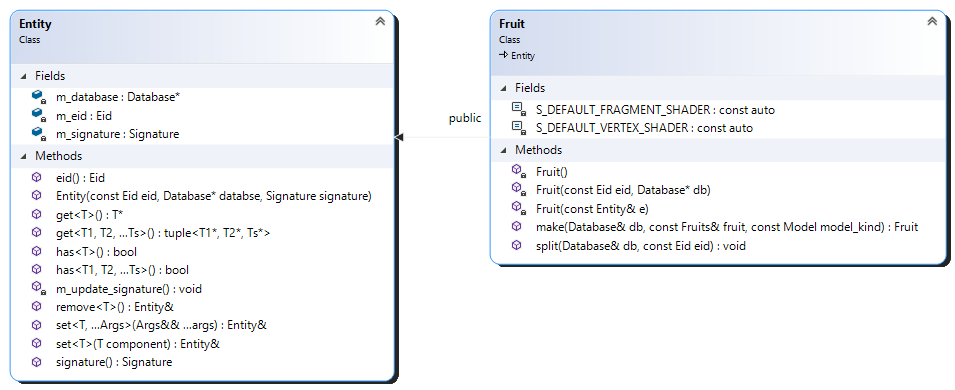
\includegraphics[width=0.95\linewidth]{images/ch20/5}
	\caption{Diagramma UML delle classi Entity e Fruit}
	\label{fig:5}
\end{figure}



\subsection{Componenti}
\marginnote{Tutte le componenti si trovano sotto il \cppinline{namespace C}.}
In fnGL un component è una qualsiasi struct/class che estende \cppinline{struct} \cppinline{Component<T>} ed è inizializzabile tramite initialization list. Le componenti, per garantire la località dei dati dovrebbero essere dei POCO\footnote{Cioè dei 
Plain Old C++ object ovvero delle semplici classi o struct che memorizzando lvalue di tipi primitivi o aggregati di primitivi.} il cui contenuto è il dato stesso e non un puntatore o un reference. 

\begin{figure}[!htp]
	\centering
	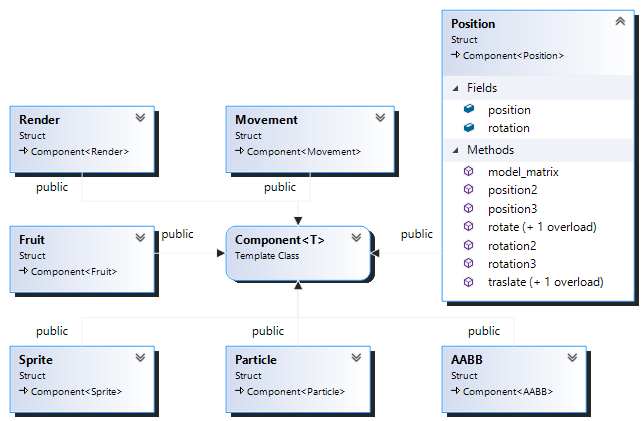
\includegraphics[width=0.95\linewidth]{images/ch20/6}
	\caption{Diagramma UML di tutte le componenti implementate in fnGL. Come è possibile vedere dal dettaglio di \texttt{C::Position} oltre ai dati in realtà possono essere presenti anche dei semplici metodi per la loro manipolazione.}
	\label{fig:6}
\end{figure}

\subsubsection{fn::Cid e fn::Signature}
Ogni component è identificata da un \cppinline{fn::Cid} anche in questo caso un intero ma memorizzato per convenienza come un \cppinline{std::bitset<N>} nel quale ogni bit è associato una componente.\sidenote{Il valore \texttt{N} deve essere almeno pari al numero massimo di components; in fnGL si utilizza 32.} In questo modo, i Cid possono essere usati in \cppinline{or} o in \cppinline{and} per semplificare di molto le operazioni del database. La riduzione in \cppinline{or} di uno o più Cid  delle componenti di un'entità è chiamata \cppinline{fn::Signature} (o firma).

\begin{cpp}[caption={
		Tutti i Cid delle varie componenti sono generati durante la compilazione in contemporanea con la risoluzione de template da parte del compilatore.  
	}, captionpos=t]
 namespace C {
     struct Position : public Component<Position> { ... };
     // Position.Cid  -->  0000 0000 0000 0001  
     struct Movement : public Component<Movement> { ... };
     // Movement.Cid  -->  0000 0000 0000 0010  
     ...
     struct AABB : public Component<AABB> { ... };
     // AABB.Cid  -->  0000 0000 0100 0000
 }  
\end{cpp}

Tutti i \cppinline{fn::Cid} sono calcolati automaticamente a compilation-time insieme alla definizione del componente; la signature (oltre che a run-time) può essere calcolata a compilation-time ricorrendo alla template variable \cppinline{Sign<...Ts>}.

\begin{cpp}[caption={
		Anche le Sign sono generate durante la compilazione. In ogni caso è comunque possibile a runtime effettuare esplicitamente operazioni manipolazione dei singoli Cid.
	}, captionpos=t]
	fn::Sign<C::Position> // -->  0000 0000 0000 0001  
    auto a = fn::Sign<C::Position, C::Movement>
    // a  -->  0000 0000 0000 0011
    auto b = fn::Sign<C::AABB, C::Movement>
    // b  -->  0000 0000 0100 0010 
    auto c = fn::Sign<C::AABB, C::Movement, C::Position, C::Fruit>
    // c  -->  0000 0000 0100 1011 
\end{cpp}

\subsubsection{\texttt{C::Position}}
La componente \cppinline{C::Position} contiene tutte le informazioni necessarie all'individuazione di un'entità nello spazio. Oltre a ciò sono anche implementati dei metodi di utility come \cppinline{translate(const glm::vec3\&)} e \cppinline{rotate(const glm::vec3\&)}.
\begin{cpp}
struct Position : public fn::Component<Position> {
	glm::vec3 position;       // Vettore posizione dell'entità
	glm::vec3 rotation;       // Rotazione (angoli di eulero) 
	...
};
\end{cpp}
Le coordinate sono espresse secondo il sistema mondo mentre la rotazione è espressa utilizzando gli angoli di Eulero\sidenote{L'utilizzo di quaternioni non è stato necessario.} riferiti ai tre assi canonici.

\subsubsection{\texttt{C::Movement}}
La componente \cppinline{C::Movement} contiene tutte le informazioni necessarie a calcolare il movimento\sidenote{Il vettore accelerazione è stato volutamente trascurato.} di un'entità nello spazio. Oltre a ciò sono anche implementati dei metodi di utility per la manipolazione basilare dei dati come \cppinline{accelerate(const glm::vec3\&)} che semplicemente incrementa la velocità.
\begin{cpp}
 struct Movement : public fn::Component<Movement> {
	 glm::vec3 velocity;   // Vettore velocità dell'entità
	 glm::vec3 spin;       // velocità angolare (angoli di eulero) 
	 ...
};
\end{cpp}
La velocità è espressa secondo il sistema mondo e la velocità angolare è utilizza gli angoli di Eulero riferiti ai tre assi canonici.



\subsubsection{\texttt{C::Render}}
La componente \cppinline{C::Render} contiene tutte le informazioni necessarie disegnare un'entità tridimensionale.
\begin{cpp}
 struct Render : public fn::Component<Render> {
     ShaderSP shader;
     ModelSP model;
 };
\end{cpp}
Dove \texttt{shader} e \texttt{model} sono due \cppinline{std::shared\_ptr} il primo allo shader che si vuole utilizzare per disegnare e l'altro al modello da disegnare.


\subsubsection{\texttt{C::Fruit}}
La componente \cppinline{C::Fruit} contiene tutte le informazioni relative ad un frutto.
\begin{cpp}
 struct Fruit : public fn::Component<Fruit> {
     Fruits fruit;
     Fruits::Model model_kind;
 };
\end{cpp}
Dove \texttt{fruit} è il frutto in questione (uno fra i possibili a disposizione) e \texttt{model\_kind} è un enum che ne specifica la tipologia che può essere: 
\begin{itemize}
	\item \texttt{whole} per indicare il frutto intero non affettato; 
	\item \texttt{half\_front} o \texttt{half\_back} per indicare una delle due metà del frutto affettato.
\end{itemize}


\subsubsection{\texttt{C::Sprite}}
La componente \cppinline{C::Sprite} contiene tutte le informazioni necessarie disegnare un'entità bidimensionale.
\begin{cpp}
 struct Sprite : public fn::Component<Sprite> {
	 SpriteSP sprite;
 };
\end{cpp}
Dove \texttt{sprite} è uno \cppinline{std::shared\_ptr} allo sprite\sidenote{ Uno sprite non è altro che una mesh bidimensionale quadrata a cui è stata applicata una texture.} da disegnare. 

\subsubsection{\texttt{C::Particle}}
La componente \cppinline{C::Particle} contiene tutte le informazioni necessarie disegnare un'entità temporanea, che appare e scompare con un' animazione di fade.
\begin{cpp}
 struct Particle : public fn::Component<Particle> {
     core::seconds lifetime;
     core::seconds elapsed;
     std::function<float(float)> interpolator;
 };
\end{cpp}
Dove \texttt{lifetime} e \texttt{elapsed} sono rispettivamente il tempo di vita della particella ed il tempo trascorso dalla sua creazione, quando \texttt{elapsed > lifetime} l'entità dovrebbe essere distrutta. 
L'attributo \texttt{interpolator} è invece un puntatore ad una funzione $f$ interpolante\sidenote{$f$ deve essere una funzione del tipo $ f:[0,1]\mapsto[0,1] $} da utilizzare per calcolare l'animazione di fade al trascorrere del tempo. 

Nella figura \ref{fig:f-function} sono mostrati i grafici di tre delle funzioni $f$ implementate:
\begin{itemize}
	\item A base gaussiana - \cppinline{asset::anim::gaussian(const float t)};
	\item Cubica di Bézier -  \cppinline{asset::anim::bezier(const float t)};
	\item A base coseno -  \cppinline{asset::anim::cosine(const float t)};
\end{itemize}

\begin{figure}[!htp]
	\centering
	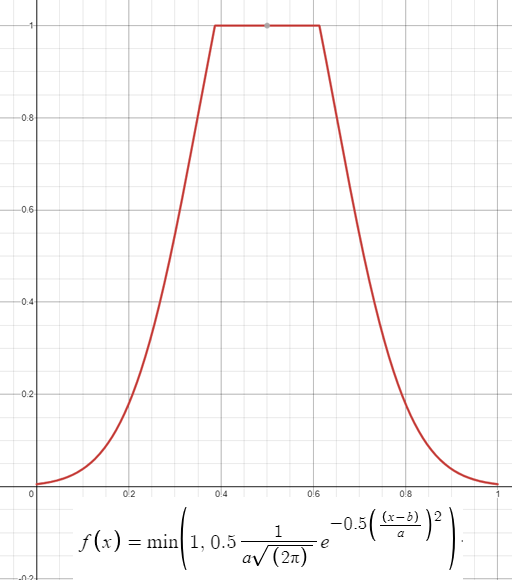
\includegraphics[width=0.32\linewidth]{images/ch20/7a} \hfill
	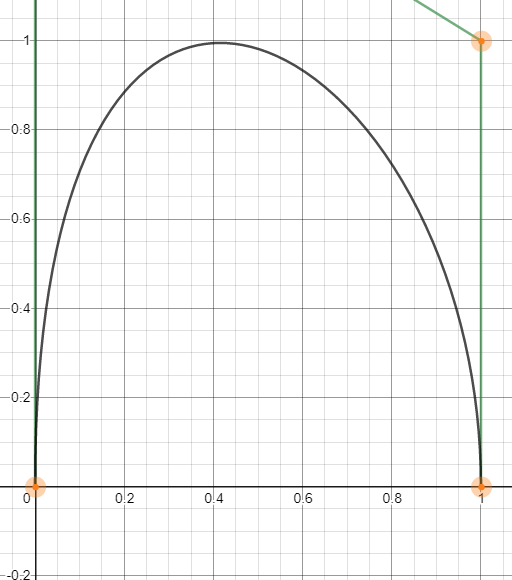
\includegraphics[width=0.32\linewidth]{images/ch20/7b} \hfill
	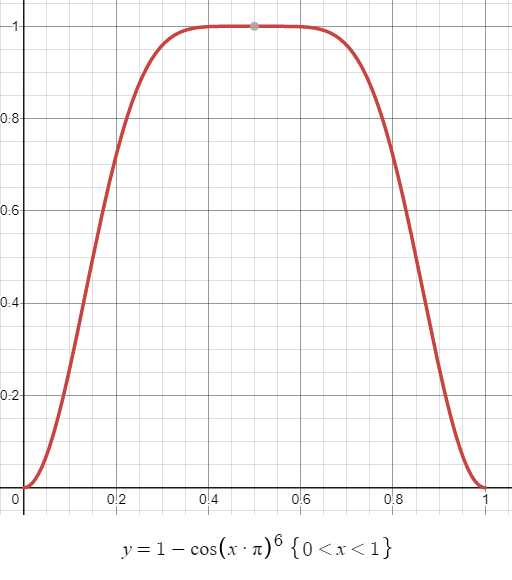
\includegraphics[width=0.32\linewidth]{images/ch20/7c} 
	\caption{Grafici delle tre funzioni interpolabili disponibili negli asset ed utilizzate all'interno del gioco. La scelta di una piuttosto che dell'altra dipende dalla velocità di animazione ricercata nelle due fasi di fade-in e fade-out.}
	\label{fig:f-function}
\end{figure}

\subsubsection{\texttt{C::AABB}}
La componente \cppinline{C::AABB} contiene l'axis-aligned bounding box (AABB) dell'entità necessario al calcolo delle collisioni.
\begin{cpp}
 struct AABB : public fn::Component<AABB> {
     glm::mat2x3 box;
 };
\end{cpp}
Dove \texttt{box} è una matrice le cui colonne sono le coordinate in sistema model dei due estremi (top-left e bottom-right) necessari a definire il box. Si è scelto di utilizzare una matrice per facilitare operazioni di trasformazione delle coordinate.

\subsection{Sistemi}
\marginnote{Tutti system si trovano nel \cppinline{namespace S}.}
In fnGL un system è una qualsiasi struct/class che estende la classe base \cppinline{System}. I sistemi implementano tutte le logiche di gestione, aggiornamento ed eventualmente rendering delle entità, ognuno di essi è applicato a tutte le entità che rispettano i requisiti di componenti del sistema.

\begin{figure}[!htp]
	\centering
	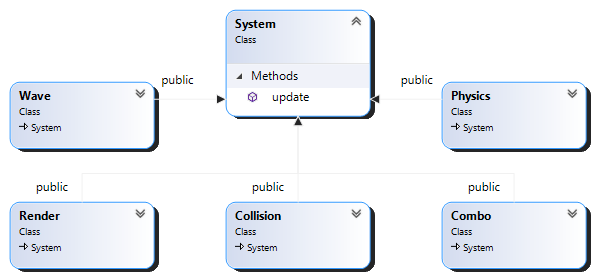
\includegraphics[width=0.95\linewidth]{images/ch20/8}
	\caption{Diagramma UML di tutti sistemu implementate in fnGL.}
	\label{fig:uml-system}
\end{figure}


\begin{exampleBox}
	Il sistema \texttt{S::Physics} gestisce la fisica del gioco relativa al movimento delle entità applicando anche l'{} accelerazione gravitazionale $g$. Per funzionare è necessario:
	\begin{itemize}
		\item la componente \texttt{C::Movement} per calcolare i nuovi vettori velocità applicando $g$;
		\item la componente \texttt{C::Position} per calcolare la nuova posizione.
	\end{itemize}
    Dunque, ad ogni update \texttt{S::Physics} effettua una query per determinare tutti quelle entità con entrambe le componenti\sidenote{Ovvero almeno con la signature \texttt{fn::Sign<C::Position, C::Movement>}.} a applica a ciascuan di esse la sua logica interna di aggiornamento.
\end{exampleBox}


\subsubsection{\texttt{S::Physics}}
Il sistema \cppinline{S::Physics} consente di gestire lo stato fisico delle entità aggiornandone posizione, rotazione, velocità e rendendoli soggetti alla forza gravitazionale. La classe ha anche il compito di eliminare quelle entità che a causa della gravità escono dallo schermo. 

I componenti coinvolti dal sistema sono: \cppinline{C::Position} e \cppinline{C::Movement}.



\subsubsection{\texttt{S::Collision}}
Il sistema \cppinline{S::Collision} si occupa di gestire ciò che avviene quando due oggetti collidono. implementando sia la rilevazione che la risposta alla collisione. I componenti coinvolti dal sistema sono: \cppinline{C::Position}, \cppinline{C::Movement},\\ \cppinline{C::AABB} e \cppinline{C::Fruit}. Nel gioco originale le collisioni non erano gestite in alcun modo.

Le collisioni sono calcolate soltanto per le entità dotate delle precedenti quattro componenti ristrette ulteriormente ai soli frutti interi\sidenote{Per scelta i frutti già tagliati sono intangibili.}. 

\subsubsubsection{Rilevamento delle collisioni}
Il rilevamento delle collisioni avviene utilizzando un approccio ibrido fra OOB e la semplice sfera.
\begin{enumerate}
\item Al momento del caricamento del modello, viene calcolata anche la AABB relativa alle sue coordinate model.
\item Durante il check delle collisioni al AABB viene trasformata in OOB applicando le stesse trasformazioni di modellazione dell'entità al box.
\item A partire da questo nuovo box viene calcolato il raggio della sfera centrato nel centro tangente al suo lato più lungo. Il raggio individua una sfera che sarà utilizzata per la rilevazione.
\end{enumerate}
Si è scelto questo approccio perché semplice e si adatta bene con la quasi totalità dei frutti i quali sono piuttosto tondeggianti.

\subsubsubsection{Risposta alle collisioni}
Quando due frutti collidono, la risposta alla collisione cerca di imitare gli urti elastici della fisica classica. In particolare, si tiene conto delle velocità iniziali e della massa dei frutti per calcolare le velocità relative a seguito dell'impatto. La formula utilizzata è:
\begin{equation}
{\begin{aligned}\mathbf {v} '_{1}&=\mathbf {v} _{1}-{\frac {2m_{2}}{m_{1}+m_{2}}}\ {\frac {\langle \mathbf {v} _{1}-\mathbf {v} _{2},\,\mathbf {x} _{1}-\mathbf {x} _{2}\rangle }{\|\mathbf {x} _{1}-\mathbf {x} _{2}\|^{2}}}\ (\mathbf {x} _{1}-\mathbf {x} _{2}),\\\mathbf {v} '_{2}&=\mathbf {v} _{2}-{\frac {2m_{1}}{m_{1}+m_{2}}}\ {\frac {\langle \mathbf {v} _{2}-\mathbf {v} _{1},\,\mathbf {x} _{2}-\mathbf {x} _{1}\rangle }{\|\mathbf {x} _{2}-\mathbf {x} _{1}\|^{2}}}\ (\mathbf {x} _{2}-\mathbf {x} _{1})\end{aligned}}
\end{equation}
Dove $\mathbf{x}_1$ e $\mathbf{x}_2$ sono i centri dei due oggetti al momento dell'impatto, $\mathbf{v}_1$ e $\mathbf{v}_2$ le velocità dei frutti ed in fine $m_1$ e $m_2$ le loro masse.


\subsubsection{\texttt{S::Wave}}
Il sistema \cppinline{S::Wave} gestisce il lancio di frutti, raggruppandoli in ondate di vario tipo e stabilendo i tempi di lancio. I componenti coinvolti dal sistema sono: \cppinline{C::Position}, \cppinline{C::Movement} e \cppinline{C::Fruit}.

Sono stati implementati quattro ``pattern di lancio":
\marginnote{Tutti i frutti compaiono sempre dal lato basso dello schermo.}
\begin{enumerate}
\item \cppinline{WaveType::RANDOM}: nel quale le componenti dell'entità sono tutte generate casualmente.
\item \cppinline{WaveType::LEFT\_TO\_RIGHT} o \cppinline{WaveType::RIGHT\_TO\_LEFT}: nel quale vengono lanciati in sequenza da sinistra verso destra (o viceversa) più frutti dello stesso tipo.
\item \cppinline{WaveType::SPOT}: nel quale avvengono lanci veloci di frutti dello stesso tipo da posizioni casuali.
\end{enumerate}

\subsubsection{\texttt{S::Combo}}
Il sistema \cppinline{S::Combo} gestisce le combo e i blitz quando si affettano più frutti in rapida successione con un solo swipe.
I componenti coinvolti dal sistema sono \cppinline{C::Sprite} e \cppinline{C::Particle}.


\subsubsection{\texttt{S::Render}}
Il sistema \cppinline{S::Render} disegna le entità tridimensionali e bidimensionali.
I componenti coinvolti dal sistema sono: \cppinline{C::Position} e \cppinline{C::Render} per gli oggetti tridimensionali e \cppinline{C::Sprite} per quelli bidimensionali.

Il rendering avviene in due fasi, prima si disegnano i modelli 3D e poi quelli 2D.




\subsection{Esempio di utilizzo}
\label{ssec:example-ecs}
Creiamo ad esempio tre entità \texttt{e1}, \texttt{e2} ed \texttt{e3} a partire da una istanza di un \cppinline{fn::Database db} nel quale i vari componenti sono già registrati.

\begin{cpp}
 fn::Entity e1 = db.create();
 fn::Entity e2 = db.create();
 fn::Entity e3 = db.create();
\end{cpp}

Le tre entità adesso sono vuote e non hanno associato alcuna componente.

\subsubsection{Set delle componenti}
Una componente può essere aggiunta ad una \cppinline{E::Entity} in due modi tramite il database ed il suo Eid oppure tramite i suoi metodi.
\begin{cpp}[caption={
		Il \texttt{set} può avvenire passando una initialization list, i parametri da inoltrare al costruttore o un oggetto componente.
	}, captionpos=t]
 // set attraverso E::Entity
 e1.set<C::Position>({});   //Costruttore di default
 e1.set<C::Movement>({		//Init list
 	.velocity=glm::vec3(1.5f, 3.6f, 9.1f),
 	.spin=glm::vec3(3.14f, -1.21f, -0.1f),
 });
 e1.set<C::Fruit>({ ... });

 e2.set<C::Position>({}); //Costruttore di default

 // set attraverso fn::Database
 db.set<C::Position>(e3.Eid, {
    .velocity=glm::vec3(1.5f, 3.6f, 9.1f),
    .spin=glm::vec3(3.14f, -1.21f, -0.1f),
 });
\end{cpp}


\subsubsection{Get delle componenti}
Con le stesse modalità del \texttt{set} è anche possibile accedere alle componenti usando la funzione \texttt{get}. Il valore ritornato è sempre un puntatore alla componente. In aggiunta è possibile anche accedere a più componenti insieme, il valore ritornato in questo caso è una \texttt{std::tuple} di puntatori.
\begin{cpp}[caption={
		Utilizzando le funzionalità di un-packing introdotte in c++17 l'utilizzo delle tuple
		risulta molto meno verboso e conveniente. Di fatto l'accesso \enquote{classico} non
		è mai utilizzato.
	}, captionpos=t]
 // get di una singola componente
 auto* p = e1.get<C::Position>();
 
 // get di più componenti classico
 auto t = e1.get<C::Position, C::Movement, C::Fruit>();
 std::get<1>(t)->accelerate(...); //--> C::Movement
 
 // get di più componenti con un-pack (c++17)
 auto [p, m, f] = e1.get<C::Position, C::Movement, C::Fruit>();
 m->accelerate(...); //--> C::Movement
\end{cpp}

\subsubsection{Controllo delle componenti}
Con le stesse modalità del \texttt{get} si può controllare se un'entità ha una o componenti utilizzando il metodo \texttt{has}.
\begin{cpp}
bool a = e1.has<C::Movement, C::Fruit>(); //true 
bool a = e2.has<C::Sprite>(); //false  
\end{cpp}



\subsubsection{Query}
Le query del database possono essere effettuate solo su un oggetto database e in due modi:
\begin{itemize}
\item Usando il metodo \cppinline{Database::having<>} che semplicemente ritorna un vettore\sidenote{questo metodo in realtà non è mai usato nella pratica.} di eid che rispettano la query.
\item Usando il metodo \cppinline{Database::for\_each<>} in combinazione con una funzione lambda che viene applicata ad ogni entità che rispetta la query.
\end{itemize}

\begin{cpp}[caption={
		I vari metodi sono in realtà tutti equivalenti dal punto di vista funzionale, da quello delle performace invece l'iterazione su un sottoinsieme di componenti è sicuramente la scelta migliore.
		\\\\
		Un'ulteriore vantaggio di questo approccio è la possibilità di creare lambda (ad esempio all'interno di eventi di gioco) da applicare alle entità.
	}, captionpos=t]
 // (a) lambda sugli eid
 db.for_each<C::Movement, C::Fruit>([](fn::Eid e){
	// fai qualcosa con e	
 }); 

 // (b) lambda sugli E::Entity
 db.for_each<C::Fruit>([](E::Entity& e){
	// fai qualcosa con e
 }); 
 
 // (c) lambda sui componenti
 db.for_each<C::Position, C::Movement>([](C::Position& p, 
                                          C::Movement& m){
	// fai qualcosa con p ed m
 }); 

 // (c) lambda sui componenti + E::Entity
 db.for_each<C::Sprite>([](E::Entity& e, C::Sprite& s){
	// fai qualcosa con e ed s
 }); 
\end{cpp}





\section{OpenGL}
Questa sezione è dedicata alle classi, funzioni e metodi che sono stati utilizzati per astrarre le primitive di OpenGL combinandole in un API che ne consenta un uso più semplice, componibile e di alto livello.

\subsection{Texture}
La classe \texttt{Texture} gestisce il caricamento, binding e generazione delle texture 2D\sidenote{Le texture 1D o 3D non sono state supportate.} in fnGL. Ogni istanza della classe rappresenta una texture caricata ed è dunque considerata come un asset e gestita dall'AssetManager.
\begin{cpp}
 Texture(const fs::path& texpath, 
         const Texture::Type type = Texture::Type::diffuse, 
         const Texture::Parameteri& parameteri = {});
\end{cpp}
Il costruttore è molto semplice e richiede del caso minimo soltanto il percorso \texttt{texpath} al file immagine contenente la texture; opzionalmente è possibile specificare anche la tipologia di texture (diffuse o specular) e i parametri della texture che saranno passati a \texttt{glTexParameteri}.

L'argomento opzionale \cppinline{Texture::Parameteri parameteri} del costruttore è un alias per \cppinline{std::unordered\_map<GLint, GLint>} utilizzabile per specificare le coppie (key, value) dei parametri. In caso di map vuota verranno utilizzati:
\begin{cpp}
 Texture::Parameteri m_parameteri = {
	{ GL_TEXTURE_WRAP_S, GL_MIRRORED_REPEAT },
	{ GL_TEXTURE_WRAP_T, GL_MIRRORED_REPEAT },
	{ GL_TEXTURE_MIN_FILTER, GL_LINEAR_MIPMAP_LINEAR },
	{ GL_TEXTURE_MAG_FILTER, GL_LINEAR },
 };
\end{cpp} 

\subsubsection{Caricamento e creazione delle texture}
Tutto il lavoro di caricamento delle texture avviene in fase di costruzione dell'oggetto da parte del metodo protected \texttt{Texture::load()} il cui codice è mostrato nel listing sottostante.

\begin{cpp}[caption={Funzione utilizzata per il caricamento, generazione e creazione delle texture in OpenGL.}, captionpos=t]
void Texture::load(){
	stbi_set_flip_vertically_on_load(true);
	
	auto f = this->m_path.string();
	unsigned char* image = stbi_load(f.c_str(), &m_width, 
                                     &m_height, 0, STBI_rgb_alpha);
	if (image == nullptr)
		fn::log::error("[ERRORE] Errore durante il load della \
		                texture {} <image=nullptr>\n", f);
	
	GL_CHECK(glGenTextures(1, &m_id));
	// Eseguo il binding della texture
	GL_CHECK(glBindTexture(GL_TEXTURE_2D, m_id));
	// Setto i parametri 
	for (auto& [key, value] : m_parameteri) {
		GL_CHECK(glTexParameteri(GL_TEXTURE_2D, key, value));
	}
	// Carico i dati della texture
	GL_CHECK(glTexImage2D(GL_TEXTURE_2D, 0, GL_RGBA, m_width,
	                      m_height, 0, GL_RGBA, 
                          GL_UNSIGNED_BYTE, image));
	// Genero eventuali mipmap
	GL_CHECK(glGenerateMipmap(GL_TEXTURE_2D));
	// Pulizia e free
	GL_CHECK(glBindTexture(GL_TEXTURE_2D, 0));
	stbi_image_free(image);
}
\end{cpp}

La prima cosa che ovviamente è necessario fare è caricare i dati detta texture dal file specificato che avviene utilizzando la image-loading library \texttt{stb\_image.h} \cite{STB}. Successivamente, è necessario chiedere ad OpenGL di generare una nuova texture, attivarla eseguendo il binding ed infine settare i parametri. 

Fatto ciò si può procedere a caricare i dati\sidenote{Fino a questo momento i dati si trovano nella memoria ram, con il seguente caricamento verranno trasferiti nella vram.} della texture e a generare eventuali mipmap necessarie.

\subsection{Mesh}
La classe \texttt{Mesh} astrae il concetto di mesh, ovvero rappresenta un reticolo poligonale che definisce un oggetto nello spazio, la rappresentazione avviene mediante vertici, indici e texture. Nei vertici sono contenuti i dati dell'oggetto mentre negli indici contengono l'adjacency information cioè come i vertici sono connessi per formare gli spigoli e le facce della mesh.

\subsubsection{I Vertex}
Per poter creare una mesh è prima necessario definire i vertici. In OpenGL un vertice è molto più di un punto nello spazio, esso può infatti contenere informazioni aggiuntive quali, nomali, coordinate texture, colori, tangenti, bitangenti etc... necessarie rendering avanzato\sidenote{Ad esempio per le luci, ombre, bumps, colori.} degli oggetti. 

L'insieme di tali informazioni insieme al loro ordine e offset all'interno del vertici è detto \textbf{Vertex Layout} che ovviamente può essere dinamico e deve essere specificato ad OpenGL. In fnGL il layout è molto semplice:
\begin{cpp}[caption={Nel vertice si memorizzano la posizione in coordinate model, la normale al vertice per l'illuminazione e le coordinate texure per appunto applicare la texture.}, captionpos=t]
struct Vertex{
	glm::vec3 position;    // Vettore posizione del vertice in coordinate model.
	glm::vec3 normal;      // Vettore normale al vertice
	glm::vec2 texCoords;   // Coordinate del vertice sulla texture
};
\end{cpp}

\subsubsection{Adjacency information}
I vertici da soli non sono sufficienti alla rappresentazione di una mesh e devono essere affiancati dall'{}adjacency information. Si tratta di una serie di indici che specificano terne (o quaterne) di vertici che formano le varie facce\sidenote{In questo modo si evita di memorizzare più volte uno stesso vertici quando si disegnano facce adiacenti ed in oltre è possibile renderizzare sottoinsiemi o definire i lati delle facce a seconda dell'ordine degli indici.} della mesh. 


\subsubsection{Caricamento e creazione delle mesh}
Il caricamento delle mesh avviene con le stesse modalità descritte per le texture nella sezione precedente. 
\begin{enumerate}
\item Si chiede ad OpenGL di generare un \textbf{VAO} (Vertex Array Object) che rappresenterà la nostra mesh sulla GPU.
\item Una volta fatto il bind del VAO si generano i due buffer che conterranno i vertici e gli indici e si procede a caricare tali informazioni:
\begin{itemize}
	\item \textbf{VBO} (Vertex Buffer Object) è il buffer di memoria che conterrà i dati dei vertici.
	\item \textbf{EBO} (Element Buffer Object) è il buffer di memoria che conterrà gli indici.
\end{itemize}
\item Una volta caricati i dati è necessario però specificare il layout dei vertici\sidenote{Ovvero dire ad OpenGL come deve interpretare i dati nel VBO che per ora è un semplice puntatore ad un blocco di byte.\\\\Per l'EBO a meno di specifiche diverse OpenGL assume che il buffer abbia valori innteri su 4Byte.}
La specifica avviene richiamando per ogni attributo del vertice la funzione \texttt{glVertexAttribPointer} specificando dimensione ed offset di partenza.
\end{enumerate}
Il codice esatto non verrà riportato per motivi di spazio.

Un'altro elemento da tenere in considerazione in questa fase è il parametro \texttt{usage} dato insieme al caricamento dei dati. Si tratta di un hint che specifica il pattern di utilizzo atteso di quei buffer per effettuare ottimizzazioni particolari quando ad esempio i dati sono statici o in stream.
\\
In fnGL tutte le mesh sono statiche, una volta caricate non vengono più modificate dunque si è utilizzato il paramtreo \texttt{GL\_STATIC\_DRAW}.


\subsection{Model}
La classe \texttt{Model} astrae il concetto di Modello 3D definito come una composizione di più mesh, solitamente infatti un modello complesso è composto da più mesh e texture. La classe inoltre implementa anche metodi per il caricamente dei modelli utilizzando la libreria ASSIMP.

\marginnote{In realtà, la struttura ad albero è solo logica, tutti i dati si trovano nell'aiScene sottoforma di array, gli altri nodi contengono solo gli indici di accesso a tali dati (ciò consente una maggiore compressione ed evita ripetizioni.)}
La libreria ASSIMP legge il file contenente il modello 3D e lo memorizza internamete in una struttura ad albero; La radice è sempre un nodo del tipo \texttt{aiScene} e contiene tutte le informazioni base e metadati sul modello 3D, la scena può avere dei sottonodi del tipo \texttt{aiNode} che a loro volta possono avere dei sottonodi del tipo \texttt{aiMesh} contenenti le mesh.

\texttt{Model} dunque oltre a comporre più mesh fa da adapter fra la classe \texttt{Mesh} di fnGL e quella di ASSIMP.

\subsection{Shader}
La classe \texttt{Shader} consente di gestire in maniera semplificata alcuni aspetti degli Shader di OpenGL. In particolare:
\begin{enumerate}
	\item Lettura, compilazione e link dei file sorgente \texttt{.glsl} della coppia vertex shader e fragment shader.
	\item Attivazione (e disattivazione) degli shader
	\item Set delle uniform con un'interfaccia polimorfica basata su template.
\end{enumerate}

Gli shader consentono di programmare la pipeline grafica manipolando i dati di vertici e texture. In fnGL sono stati implementati 4 tipi di shader per gestire altrettante esigenze di rappresentazione. 


\subsubsection{Picking shader}
È quello più semplice, il suo scopo è disegnare un oggetto con un unico colore flat; senza luci, ombre o texture. Tale colore identificando univocamente l'oggetto disegnato e potrà essere utilizzato per implementare il picking. 

Il Vertex Shader disegna semplicementge i vertici dell'oggetto secondo la model-view-projection.
\begin{cpp}[caption={Codice sorgente del Vertex Shader. Applica la trasformazione a tutti i vertici del modello.}, captionpos=t]
 #version 330 core
 layout ( location = 0 ) in vec3 position;
 layout ( location = 1 ) in vec3 normal;
 layout ( location = 2 ) in vec2 texCoords;

 uniform mat4 model;
 uniform mat4 view;
 uniform mat4 projection;
 
 void main( )
 {
     gl_Position = projection * view * model * \
 	               vec4( position, 1.0f );
 }
\end{cpp}

Il Fragment Shader disegna con un unico colore (\texttt{r}, \texttt{g}, \texttt{b}, \texttt{a}) l'oggetto.
\begin{cpp}[caption={Codice sorgente del Fragment Shader.}, captionpos=t]
 #version 330
 
 uniform int r;
 uniform int g;
 uniform int b;
 uniform int a;
 
 out vec4 outputF;
 
 void main()
 {
     outputF = vec4(r/255.0, g/255.0, b/255.0, a/255.0);
 }
\end{cpp}




\subsubsection{Blade shader}
È lo shader utilizzato per rappresentare la ``blade" ovvero la lama mostrata quando si scorre con il mouse per tagliare i frutti. 

Il Vertex Shader è simile a quello della sezione precedente, l'unica differenza è il ``forward" delle coordinate texture allo shader successivo in modo che possa utilizzarle per disegnare la lama.
\begin{cpp}[caption={Codice sorgente del Vertex Shader. Applica la trasformazione a tutti i vertici del modello e ritorna le coordinate texture.}, captionpos=t]
 #version 330 core
 layout ( location = 0 ) in vec3 position;
 layout ( location = 1 ) in vec3 normal;
 layout ( location = 2 ) in vec2 texCoords;
 
 out vec2 TexCoords;
 
 uniform mat4 model;
 uniform mat4 view;
 uniform mat4 projection;
 
 void main( )
 {
 	gl_Position = projection * view * model * \ 
 	              vec4( position, 1.0f );
 	TexCoords = texCoords;
 }
\end{cpp}



Il fragment shader utilizza le coordinate texture per determinare il colore dei pixel della mesh. Le coordinate sono interpolate con un sampler2D che dipende dai parametri specificati alla creazione della texture. 
\begin{cpp}[caption={Codice sorgente del Fragment Shader.}, captionpos=t]
 #version 330 core
 
 in vec2 TexCoords;
 out vec4 color;
 
 uniform sampler2D texture_diffuse;
 
 void main( )
 {
 	color = vec4( texture( texture_diffuse, TexCoords ));
 }
\end{cpp}

Le lame implementate hanno texture bicolore e per ottenere bordi netti è necessario utilizzare \texttt{GL\_NEAREST}.

\begin{figure}[!htp]
	\centering
	
\includegraphics[width=0.2\linewidth]{images/ch20/blade0}
	$\quad$
	
\includegraphics[width=0.2\linewidth]{images/ch20/blade1}
	$\quad$
	
\includegraphics[width=0.2\linewidth]{images/ch20/blade2}
	$\quad$
	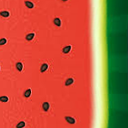
\includegraphics[width=0.2\linewidth]{images/ch20/blade3}
	\caption{Esempio delle tre texture disponibili per le lame. Tutte e quattro derivano da lame realmente esistenti all'interno del gioco.}
	\label{fig:blades}
\end{figure}


\subsubsection{Sprite shader}
Questo shader può essere visto come una semplice estensione di quello usato per disegnare la lama che consente in più di specificare il canale alpha del colore della texture, in questo modo è possibile disegnare oggetti trasparenti.


\subsubsection{Fruit Shader}
Lo shader dedicato al disegno dei frutti e anche quello più complesso dal momento che oltre alle caratteristiche viste in precedenza implementa anche il lighting secondo il modello di riflessione di Phong.


Nel vertex shader oltre alla posizione dei vertici vengono definite anche:
\begin{itemize}
\item La posizione dell'unica sorgente di luce; che deve poi essere convertita in coordinate view. Si tratta di un parametro fisso.
\item Si ricalcolano le normali dei vertici rispetto la model-view.
\end{itemize} 
Queste informazioni sono poi restituite in output allo shader successivo in modo che possa calcolare secondo il modello di Phong le varie componenti della luce.

\begin{cpp}[caption={Codice sorgente del Vertex Shader. Applica la trasformazione a tutti i vertici del modello e ritorna le coordinate texture, posizione della luce e le normali.}, captionpos=t]
#version 330 core
layout (location = 0) in vec3 aPos;
layout (location = 1) in vec3 aNormal;
layout (location = 2) in vec2 aTexCoords;

out vec3 FragPos;
out vec3 Normal;
out vec3 LightPos;

out vec2 TexCoords;

uniform mat4 model;
uniform mat4 view;
uniform mat4 projection;

void main()
{
	// Posizione della luce che illumina la scena
	vec3 lightPos = vec3(0.0f, 30.0f, 30.0f);
	
	gl_Position = projection * view * model * vec4(aPos, 1.0);
	// Calcolo la posizione del fragment
	FragPos = vec3(view * model * vec4(aPos, 1.0));
	// Calcolo le normali
	Normal = mat3(transpose(inverse(view * model))) * aNormal;
	// Coord world -> coord view per la luce
	LightPos = vec3(view * vec4(lightPos, 1.0)); 
	
	TexCoords = aTexCoords;
}
\end{cpp}









Nel fragment shader infine avviene il calcolo della luce e quello del colore della texture, i due valori saranno poi combinato per ottene il colore finale. La luce scelta di base è bianca.
\begin{itemize}
\item \textbf{Luce ambientale}: È la componente ``ambientale" della luce derivante dall'ambiente circostante, gli oggetti infatti non sono mai completamente scuri. È derivata dalla luce di base utilizzando un intensità pari a \texttt{0.4}.

\item \textbf{Luce diffusa}: È la componente diffusiva della luce, che varia a seconda di come i raggi impattano sulla superficie degli oggetti e dall'angolo che si viene a creare fra superfice e sorgente. È derivata dalla luce di base attraverso sua posizione e le normali alle superfici.

\item \textbf{Luce speculare}: È la componente speculare della luce, simula i punti luminosi che si vedono quando la luce riflette su oggetti lucenti. Tale componente varia a seconda dell'angolo fra viwer, superficie e sorgente. Anch'essa è derivata dalla luce di base utilizzando un intensità\sidenote{L'utilizzo di un valore maggiore rende i frutti `plasticosi' e riduce dunque il realismo.} pari a \texttt{0.3} ed un fattore di decay di \texttt{32}.
\end{itemize}

L'unione di queste tre componenti, unite al colore del pixel derivato dalla texture consente di determinare il colore finale dell'oggetto.

\begin{cpp}[caption={Codice sorgente del Fragment shader che implementa l'illuminazione di Phong.}, captionpos=t]
#version 330 core
out vec4 FragColor;

in vec2 TexCoords;
in vec3 FragPos;
in vec3 Normal;
in vec3 LightPos;   // posizione luce in wcoord

uniform sampler2D texture_diffuse;

void main()
{
	// Colore della luce, bianco
	vec3 lightColor = vec3(1.0f, 1.0f, 1.0f);
	
	//::::::::::::::::::::::::::::::::::::::::::::::::
	//::::::  CALCOLO DELLA LUCE AMBIENTALE     :::::: 
	//::::::::::::::::::::::::::::::::::::::::::::::::
	float ambientStrength = 0.4;
	vec3 ambient = ambientStrength * lightColor;    
	
	
	//::::::::::::::::::::::::::::::::::::::::::::::::
	//::::::  CALCOLO DELLA LUCE DIFFUSA        :::::: 
	//::::::::::::::::::::::::::::::::::::::::::::::::
	vec3 norm = normalize(Normal);
	vec3 lightDir = normalize(LightPos - FragPos);
	float diff = max(dot(norm, lightDir), 0.0);
	vec3 diffuse = diff * lightColor;
	
	//::::::::::::::::::::::::::::::::::::::::::::::::
	//::::::  CALCOLO DELLA LUCE SPECULARE      :::::: 
	//::::::::::::::::::::::::::::::::::::::::::::::::
	float specularStrength = 0.3;
	float decay = 32;
	
	// versore alla visione del viewer, nel  view-space
	// il viewer sta sempre in (0,0,0)
	vec3 viewDir = normalize(-FragPos); 
	vec3 reflectDir = reflect(-lightDir, norm);  
	float spec = pow(max(dot(viewDir, reflectDir), 0.0), decay);
	vec3 specular = specularStrength * spec * lightColor; 
	
	
	// Combino i risultati con il colore della texture
	vec3 objectColor = (texture( texture_diffuse, TexCoords)).xyz;
	vec3 result = (ambient + diffuse + specular) * objectColor;
	FragColor = vec4(result, 1.0);
}
\end{cpp}